\subsection{Authorship clustering methods \label{sec:authorship_clustering_methods}}

To find clusters of authors, a possible way is to use a hierarchical clustering algorithm on a rank list.
The rank list indicate if the two documents should belong to the same cluster by order of certainty.
The hierarchical clustering regroup documents following this order.

The hardest task with this clustering scheme is to find the position in the rank list where true link become less frequent than false link.
In a the clustering context, the optimal position is unknown since the true labels are not available.
The position should minimized the true links under it and the false links above it.

In this study, finding this position will also be refered as finding the \textit{cut}.
We define the true positive as true links above the cut, true negatives as false links under the cut.
In addition false positive are true links under the cut and false negatives are false links above the cut.

To find this cut, three approaches are explored : an unsupervised, a semi-supervised and a supervised.
The unsupervised method can be used when only one corpus is available and no learning procedures can be applied.
The semi-supervised learn based on a corpus with labels (training corpus) a rank list score where the cut should be for any other corpus (called testing corpus).
Finally, the supervised approach, learn based on a rank from a corpus with labels (training corpus) a model.
The model can find the optimal cut for a rank list from a new corpus (called testing corpus) generated using the same metrics as ones used for training.

\subsubsection{Agglomerative clustering}

The scikit-learn package~\cite{sklearn} provide an implementation bottom-up implementation of the hierarchical clustering, which is called agglomerative clustering.

The agglomerative clustering follow this procedure:
\begin{enumerate}
  \item The rank list used is converted into a 2D distances' matrix with each link representing a element of the matrix (ref. ~\label{sec:distances_matrix}).
  \item At the begining, each document is considered as a single document cluster.
  \item The link (element) with the lowest score in the matrix is used to merge the next clusters.
  \item The matrix is updated following a linkage criteria.
  \item Point 3 and 4 can be repeated until a single cluster is remaining.
\end{enumerate}

Multiple linkage criteria are available : \textit{Ward} (metric that aim to minimize the variance of the cluster merged), \textit{average-linkage} (use the average score of each link of the cluster merged), \textit{complete-linkage} (use the maximal score of the cluster merged), \textit{single-linkage} (use the minimal score of the cluster merged).
Example~\ref{ex:agglomerative_clustering} show an example for the merging procedures and the linkage criteria.

Ward linkage was discarded since the current implementation only allow Euclidian distance for its computation.
The merging procedure can be stopped either of the two following criteria : When a certain number of cluster is reached or when the minimal score for the next merge is above a certain value.
This value is called the distance threshold.

The so called \textit{cut} can be associated to the distance threshold.
The cut is a position in the rank list and the distance threshold is the score which can seperate the rank list.

There is one of the main issue with the scikit-learn implementation.
It does not provide a way to access the current cluster at each merging step.
A possible workaround is to run the algorithm multiple time.
Each time the algorithm is stopped at a different number of cluster.
This workaround introduce an overhead of $O\frac{n * (n - 1)}{2} = O(n^2)$, with $n$ equal to the number of documents.
The agglomerative clustering algorithm was re-implementated to allow access to the clusters at each steps and avoid this overhead.

\begin{example}
  \small
  \centering
  \caption{Agglomerative clustering}
  \label{ex:agglomerative_clustering}

  \begin{subexample}{\linewidth}
    \centering
    \subcaption{Initial clusters and their distances}
    \begin{tabular}{c|c c c c}
      \toprule
        & A & B & C & D \\
      \midrule
      A & - & \textbf{1} & $2$ & $3$ \\
      B & - & - & $8$ & $7$\\
      C & - & - & - & $6$ \\
      D & - & - & - & - \\
      \bottomrule
    \end{tabular}
  \end{subexample}

  \vspace{0.2cm}
  The link with the smallest distance is A-B with a distance of 1.
  At the next step the clusters A and B are merged into a cluster called AB.

  \vspace{0.5cm}

  \begin{subexample}{\linewidth}
    \centering
    \subcaption{First merge using single-linkage}
    \begin{tabular}{c|c c c}
      \toprule
        & AB & C & D \\
      \midrule
      AB & - & $\text{min} \left[2, 8 \right] = 2$ & $\text{min} \left[3, 7 \right] = 3$ \\
      C  & - & - & $6$ \\
      D  & - & - & - \\
      \bottomrule
    \end{tabular}
  \end{subexample}

  \vspace{0.2cm}
  Next step will merge AB and C.

  \vspace{0.5cm}

  \begin{subexample}{\linewidth}
    \centering
    \subcaption{First merge using average-linkage}
    \begin{tabular}{c|c c c}
      \toprule
        & AB & C & D \\
      \midrule
      AB & - & $\text{avg} \left[2, 8 \right] = 5$ & $\text{avg} \left[3, 7 \right] = 4$ \\
      C  & - & - & $6$ \\
      D  & - & - & - \\
      \bottomrule
    \end{tabular}
  \end{subexample}

  \vspace{0.2cm}
  Next step will merge AB and D.

  \vspace{0.5cm}

  \begin{subexample}{\linewidth}
    \centering
    \subcaption{First merge using complete-linkage}
    \begin{tabular}{c|c c c}
      \toprule
        & AB & C & D \\
      \midrule
      AB & - & $\text{max} \left[2, 8 \right] = 8$ & $\text{max} \left[3, 7 \right] = 7$ \\
      C  & - & - & 6 \\
      D  & - & - & - \\
      \bottomrule
    \end{tabular}
  \end{subexample}

  \vspace{0.2cm}
  Next step will merge C and D.
\end{example}

\subsubsection{Unsupervised clustering \label{sec:unsupervised_clustering}}

The idea is to run the agglomerative clustering at each number of clusters (at each merge step).
When discarding clustering with $N$ and clusters $1$, this produce $N - 2$ possible clusterings, each of those can be evaluated using the mean Silhouette score.
See definition~\ref{def:silhouette}.

\begin{definition}[Mean Silhouette score~\cite{sklearn}~\cite{wiki_silhouette}]
  \label{def:silhouette}
  The mean Silhouette score is an unsupervised clustering metric which evaluate a clustering result by measuring the cohesion and separation of the clusters.
  \begin{equation}
    s = \frac{1}{|C|} \sum_{i = 0}^{|C|} \frac{b(i) - a(i)}{max(a(i), b(i))}
  \end{equation}
  \begin{equation*}
    \begin{split}
      a(i)&: \text{mean intra-cluster distance} \\
      a(i)& = \frac{1}{|C_i| - 1} \sum_{j \in C_i, i\neq j} d(i, j) \\
      b(i)&: \text{mean nearest-cluster distance} \\
      b(i)& = \min_{k\neq i} \frac{1}{|C_k|} \sum_{j \in C_k} d(i, j) \\
    \end{split}
  \end{equation*}
  With $C$ the set of clusters, $C_i$ the i-th cluster, $d(i, j)$ the distance between the document i and j.
  The value is ranged between -1 and 1, a large value indicate a good cohesion and good separation of the clusters (low intra-cluster distance, high nearest-cluster distance).
\end{definition}

The idea is to apply the hierarchical clustering at each possible number of clusters (from $N - 1$ to $2$), and compute the mean Silhouette score.
The best clustering is the one which have the largest mean Silhouette score.
An alternative to this method is the Iterative Positive Silhouette (IPS) and was proposed in Layton, Watters, Dazeley (2011)~\cite{automated_unsupervised}.

\subsubsection{Semi-supervised distance threshold selection using two Beta distributions}

In Savoy (2014)'s \textit{Estimating the Probability of an Authorship Attribution} they modelized the distribution of the true and false links across the score obtained using a mixture of 2 beta distribution~\cite{savoy_probability}.
Using these two beta distribution models, the position where the area under the curve for both models is maximized (same area under the cut for both models), correspond to the position where the true positive and true negatives are maximized.
Thus, the statistical best possible location whereto separate the rank list if we want to minimize the false positive and false negatives (non-weighted minimization errors).
The idea is to reuse this position for any new rank lists.

To find the position where both beta distribution have the same area under the curve, there might be analytical ways to solve this problematic using the \textit{beta distribution cumulative distribution function analytic form} (beta CDF, probability, area under the curve) but was ignored for this study.
Instead, the equiprobable position is found using a binary search between 0 and 1.
At each step the CDF for the two beta distribution is evaluated until it converges to the same value (or until their difference is a small value, such as $10^{-15}$).

Figure~\ref{fig:links_score_density} show the density of true and false link as well as a beta distribution estimation for St-Jean (Regression fusion in \ref{fig:links_score_density_fusion_regression} and Z-Score fusion in \ref{fig:links_score_density_fusion_z_score}).
For the metrics with a score outside the interval $[0, 1]$ (such as the Z-Score fusion), the distances have been normalized between 0 and 1 using Definition~\ref{def:normalization} to be able to modelize the beta distribution.

The results obtained by the regression fusion (ref.~\ref{sec:regression_fusion}) are a probability of being a true link, so the two distribution are well separated and can be modelized by the two beta distributions.
In the other hand, when using the Z-Score fusion, the scores are overlapping more, but can also be modelized using the two beta distributions.
As explained in~\cite{savoy_probability} the beta distribution is better suited for authorship problem than the Gaussian distribution since it can grasp a large amount of distribution shapes with its parameters' flexibility.
The vertical line indicate the equiprobable position where both beta distribution have the same probability of being a true link and false link (same area under the curve), found using the binary search.
This point can be used as a decision point where the cut should be made in the rank list, this ensures that both false positives and false negatives are minimized.
Since the authors of each document must be known to find the cut, the idea is here to find the cut location using corpus with known authors and re-use the same value for new corpora, thus turn this method into supervised.

We consider this method as semi-supervised since the only \textit{learnt} parameter is a fixed real number, the distance threshold, and this method do not consider any new corpus for this value computation.
The linkage parameter for this method is the complete linkage, since the cut correspond to the position where the most extremes of the same categories, either true or false links meet.

This technique can be adapted, in the case where the false positives do not have the same importance as false negatives.
The position search criteria can be change such that instead of finding the position where both the true link and false link area correspond to 50\% of their sum (equiprobable case).
It can be generalized such that the true link area represent $\alpha$ and the false link area to $1-\alpha$ with $\alpha \in \left[0,1\right]$.
When $\alpha$ is greater than 0.5, more false positives will occure and less false negatives and when $\alpha$ is smaller than 0.5, more false positives and more false negatives.
The same binary search can be used for this computation, just the target need to be changed.

\begin{figure}
  \caption{Links score distribution and beta distribution estimation for St-Jean}
  \label{fig:links_score_density}

  \subcaption{Regression fusion (training Oxquarry)}
  \label{fig:links_score_density_fusion_regression}
  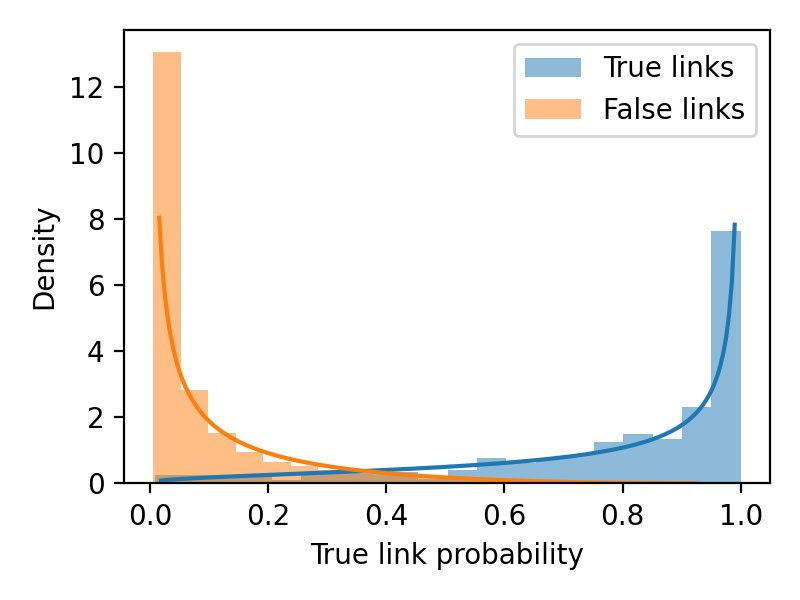
\includegraphics[width=\linewidth]{img/links_score_density_fusion_regression.png}

  \vspace{0.5cm}

  \subcaption{Z-Score fusion}
  \label{fig:links_score_density_fusion_z_score}
  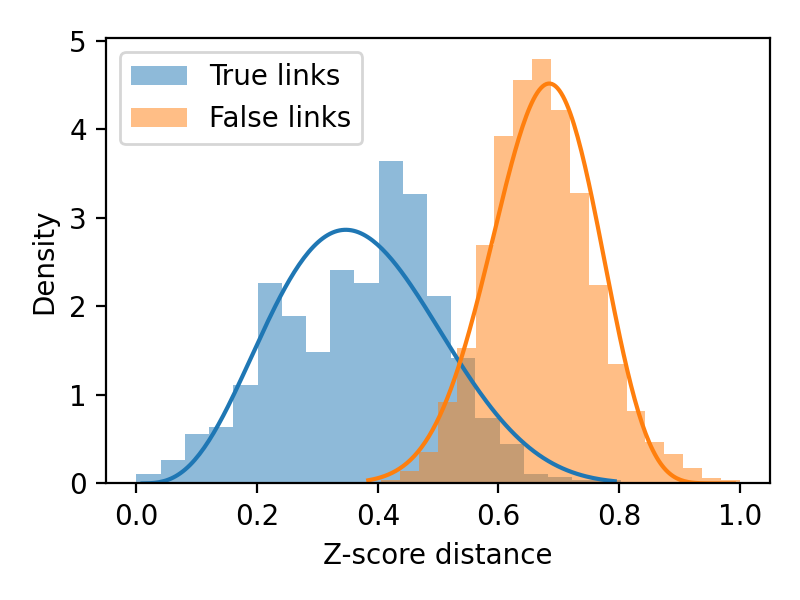
\includegraphics[width=\linewidth]{img/links_score_density_fusion_z_score.png}
\end{figure}

\subsubsection{Supervised distance threshold selection using Logistic Regression}

To learn at which position in the rank list the cut should be, this third idea is to fit a linear regression model on samples created from the rank list.
The model must be linear since only one cut should seperate the true links and the false links.
To train the model, a sample is created for each link in a rank list.
The links labels are either \textit{true} (1.0) when both document in the link are from the same author and \textit{false} (0.0) otherwise.

The features used are : the log of the relative rank ($log \frac{rank}{|L|}$) and the score of the link.
The first feature to take into account that true links are generally on the top of the rank list.
The value is normalized to be able to generalize this value to any rank list size.
The logarithm allow to have a greater contrast in value for the top rank while considering bottom rank as more or less equal.
The second feature aim to consider that the small distances are generally true links.

Using these two features, the model can grasp the importance of the rank and the score of each link.
Since the training is only based on the relative rank and the score at each rank, the trained model is language independent and size independent.
But this model is metric dependent, since the score magnitude can variate depending on the distance function.

In this study, the model used is the logistic regression.
The advantage of using a regression model is that the output of the model will correspond to a probability of being a true link according to the model.
To find the cut on the test datasets, the fitted model predict the probability of being a true link on every link in the new rank list.
From these predictions, a probability threshold must be chosen.

For example, having a probability threshold at $0.5$, minimize both false negatives and the false positives.
This can be adjusted, for example if false negatives are more important to minimize, a probability threshold at $0.6$ can be selected instead or $0.4$ if the false positive should be minimized.
For the sake of simplicity, the probability threshold chosen is $0.5$.

The distance threshold to correctly separate true links to false links is chosen by linearly interpolating the probability threshold with its closest probability of the one above and the one below to their scores.
This ensures that the distance threshold chosen is even correct between ranks for any new corpus.
Example~\ref{ex:linear_interpolation} showcase a linear interpolation computation using a probability threshold of $0.5$.
The logistic regression model can be re-used on any other rank lists produced with the same distance metrics.

\begin{example}
  \centering
  \caption{Linear interpolation for supervised distance threshold selection (probability threshold fixed at 0.5)}
  \label{ex:linear_interpolation}

  \begin{subexample}{\linewidth}
    \centering
    \subcaption{Rank list with link probability and score}
    \begin{tabular}{l r r}
      \toprule
      Rank & Probability & Score \\
      \midrule
      (...) & &\\
      45th & 0.54 & 15 \\
      46th & 0.52 & 13 \\
      47th & 0.49 & 12 \\
      48th & 0.48 & 10 \\
      (...) & & \\
      \bottomrule
    \end{tabular}
  \end{subexample}

  \vspace{0.5cm}

  \begin{subexample}{\linewidth}
    \centering
    \subcaption{Linear interpolation}
    \begin{align}
        \alpha &= \frac{0.5 - 0.49}{0.52 - 0.49} = \frac{1}{3} \\
        \textit{distance\_threshold}_{@0.5} &= (13 - 12) \cdot \alpha + 12 = 12 + \frac{1}{3}
    \end{align}
  \end{subexample}

\end{example}
